\documentclass[12pt]{memoir}

\usepackage{cdsc-memoir}
% there are two chapter styles: cdsc-article and cdsc-memo
% memo assumes that you remove the "\\" and the email address from the
% \author field below as well as that you will comment out the
% \published tag
\chapterstyle{cdsc-article}

\usepackage[utf8]{inputenc}
\usepackage{wrapfig}
\usepackage[T1]{fontenc}
\usepackage{textcomp}
\usepackage[garamond]{mathdesign}


% \textwidth = 5.2inches
\usepackage[letterpaper,left=1.65in,right=1.65in,top=1.3in,bottom=1.2in]{geometry}

% packages i use in essentially every document
\usepackage{graphicx}
\usepackage{enumerate}

% packages i use in many documents but leave off by default
\usepackage{amsmath}
% \usepackage{dcolumn}
% \usepackage{endfloat}

% import and customize urls
\usepackage[usenames,dvipsnames]{color}
\usepackage[table]{xcolor}
\usepackage{soul}
\usepackage[breaklinks]{hyperref}
\usepackage{array}
\hypersetup{colorlinks=true, linkcolor=Black, citecolor=Black, filecolor=Blue,
    urlcolor=Blue, unicode=true}
\hyphenation{com-men-sal-ism}
% list of footnote symbols for \thanks{}
\makeatletter
\renewcommand*{\@fnsymbol}[1]{\ensuremath{\ifcase#1\or *\or \dagger\or \ddagger\or
 \mathsection\or \mathparagraph\or \|\or **\or \dagger\dagger
  \or \ddagger\ddagger \else\@ctrerr\fi}}
\makeatother
\newcommand*\samethanks[1][\value{footnote}]{\footnotemark[#1]}

\DeclareRobustCommand{\myhl}[2]{\sethlcolor{#1} \hl{#2}}

% add bibliographic stuff 
\usepackage[american]{babel}
\usepackage{csquotes}
\usepackage[natbib=true, style=apa, backend=biber]{biblatex}
\addbibresource{Ecology.bib}
\DeclareLanguageMapping{american}{american-apa}

\defbibheading{secbib}[\bibname]{%
  \section*{#1}%
  \markboth{#1}{#1}%
  \baselineskip 14.2pt%
  \prebibhook}

\def\citepos#1{\citeauthor{#1}'s (\citeyear{#1})}
\def\citespos#1{\citeauthor{#1}' (\citeyear{#1})}

% memoir function to take out of the space out of the whitespace lists
\firmlists

% LATEX NOTE: these lines will import vc stuff after running `make vc` which
% will add version control information to the bottom of each page. This can be
% useful for keeping track of which version of a document somebody has:
% \input{vc}
% \pagestyle{cdsc-page-git}

% LATEX NOTE: this alternative line will just input a timestamp at the
% build process, useful for Overleaf
% \pagestyle{cdsc-page-overleaf}
\usepackage{tikz}
\usetikzlibrary{positioning,shapes,arrows,fit,chains,shapes.geometric,trees}

\definecolor{hypothesizedcell}{HTML}{a9d89c}
\definecolor{nullhypothesizedcell}{HTML}{d89ca9}
\definecolor{agnosticcell}{HTML}{9ca9d8}

\begin{document}
\renewcommand{\arraystretch}{2}
\setlength{\parskip}{4.5pt}
% LATEX NOTE: Ideal linespacing is usually said to be between 120-140% the
% typeface size. So, for 12pt (default in this document, we're looking for
% somewhere between a 14.4-17.4pt \baselineskip.  Single; 1.5 lines; and Double
% in MSWord are equivalent to ~117%, 175%, and 233%.

\baselineskip 16pt

\title{Outline for: Unpacking Ecological Approaches to Online Communities }
\author{Your Name\\
        \href{mailto:youremail@uw.edu}{youremail@uw.edu}}
\date{}

\published{\textsc{\textcolor{BrickRed}{This document is an
  unpublished draft.\\ Please do not distribute or cite without
  permission.}}}

\maketitle

\begin{abstract}
Internet researchers are increasingly aware of important interdependence between online groups.  HCI researchers have drawn density dependence theory from population ecology to theorize competitive and complementary dynamics between communities with overlapping content and participants and predict growth and survival of online groups.   Density dependence theory highlights similarities between online groups as exchangeable members of a homogeneous population while minimizing the role of diversity and the importance of specialization.   Community ecology, a complementary approach proposes that each group plays a distinctive role in the broader sociotechnical ecosystem.   Vector autoregression (VAR) models are a method from community ecology  for estimating a network of competitive, complementary, and asymmetrical commensalist relations.  We introduce community ecology to HCI research by comparing population and community ecologies, explicating applicable concepts from community ecology, and testing hypothesis using a vector autoregression model fit to time-series data from Reddit.
\end{abstract}

\section{Dissemination Objectives}

This is a dissertation chapter and a CHI 2021 paper. The CHI 2020 deadline is Sep. 10 2020 for abstracts and metadata and Sep. 17th for the submission. I aim to submit or have a solid draft before then. Let's say July 1. 

I'll release code and datasets.

There isn't a practitioner or outreach component specific to this paper. 

\section{Rationale}

\begin{itemize}
\item Accumulating empirical results demonstrate how interdependence between online groups shapes participation, growth, and survival (we use the term ``online group'' to avoid confusion with ecological communities).  Yet relatively few studies provide general methodological tools and even fewer provide general theoretical concepts for systematically studying interdependence between online groups. 

\item Ecology provides general tools for conceptualizing and modeling these relationships.  Organizational social scientists have long worked on extensions from biological ecology and influenced prior research in HCI.  We continue building ecological theorizing in the context of HCI by introducing concepts and models from community ecology.  Community ecology aims to characterize the network of relations that shift or stabilize an ecosystem and thereby gain insights into the nature of the system and how it can be regulated.  

\item Prior work in HCI tests theories of density dependence from population ecology based on overlapping users and content \citep{zhu_impact_2014,zhu_selecting_2014,wang_impact_2013}.  Population ecology places online groups in the position of the biological organism and the set of groups on an online platform occupy the position of a population of species.  This highlights the similarity of groups as members of the same populations while minimizing the diverse roles that groups can play in the online ecosystem.   Community ecology by contrast analyzes populations as distinct interdependent constituents of an ``ecological community'' \citep{astley_two_1985-1}.  Community ecology places each community in the conceptual position of a distinct biological population and seeks to understand how communities relate to one another.  

In their empirical analyses, the above studies already take steps toward a community ecology approach by modeling density dependence as structured by overlapping memberships and topics between online groups.  Rather than assuming all communities face the same environment in strict population ecology approach, each group in their analysis faces a distinct environment of overlapping groups. They use the ``niche'' concept to refer to fit between a group and it's participants and content. Yet they stop short of explicating community ecology concepts or estimating the ``community matrix'' which quantifies relations of interdependence between online communities. 

% Why are community ecology concepts useful to understanding online communities?
\item Community ecology provides concepts for how online groups relate to one another.  These can give community managers ways to think about the role of individual communities in the broader context, to help answer questions like ``How might groups about similar topics shape activity and participation in one another?'' or ``What topics might we be able to create a new group around?'', ``When will we have more small groups or few large groups?'' Community ecology can also inform design choices like whether to allow users to create new groups and the potential effects of interventions like banning, quarantining, and norms against coordinated cross-participation.

% Why do we care about estimating the community matrix?
% Why is estimating the CM a goal of community ecology?
\item Community ecology provides statistical models tools for understanding sociotechnical ecosystems.  In particular, vector autoregression (VAR) models can infer ecological networks of complementary, competitive, predatory, and communal relationships.  VAR analysis can quantify the stability of the system and affords exploration of counterfactual forecasts to simulate hypothetical interventions. 

\item Geographically local online communities are important sites in the networked public sphere where people go to make sense of current events and local concerns.  They also generate data that is relatively easy to cast into a community ecology model.  This study contributes to understanding these communities through the lens of community ecology.

\item Community ecology promises a vast depth of analysis at levels of granularity ranging from narrow ``ecological communities'' consisting of a handful of tightly related groups to estimating ecological networks for entire large platforms like Reddit.  Therefore this project will be a first step focused on translating community ecology for HCI and a demonstrative analysis.

\end{itemize}

\section{General Objectives}

\begin{itemize}
\item Provide answers to ``How does the growth/success of an online group depend on the environmental context?''  and ``How can we understand interdependence between online groups?''

\item Provide an overarching conceptual framework for studies of interdependence in social computing.

\end{itemize}

\section{Specific Objectives}
\begin{itemize}

\item Argue that community ecology is a more appropriate framework than population ecology for thinking about interdependence between online groups.

\item Build on prior use of the concept of \emph{niches} in HCI to emphasize that niche overlaps can be associated qualitatively different kinds of relationships.   

\item Define and motivate concepts of \emph{ecological community}, \emph{competition}, \emph{complementary} and \emph{commensalism} and \emph{specialization} for online communities.

\item Explicate the above concepts through testing hypotheses about when communities will compete or be complementary using \emph{resource partitioning theory} and \emph{the principle of competitive exclusion} using one or more case studies from Reddit.

\end{itemize}

\section{Propositions}

\begin{itemize}
\item \textbf{P1:} For geographic subreddits, ecological relationships between generalists will probably be competitive. That is, generalist $\rightarrow$ generalist edges will have positive coefficients in estimated community matrices. 

\item \textbf{P2:} For geographic subreddits, ecological relationships from generalist to specialists will probably be beneficial to specialists. That is, generalist $\rightarrow$ specialist edges will have positive coefficients in estimated community matrices.

\item \textbf{P3:} For geographic subreddits, ecological relationships between generalists and specialists are likely to be commensal. Sepcifically, generalist $\rightarrow$ specialist edges will have greater coefficients in estimated community matrices compared to specialist $\rightarrow$ generalist edges. 

\end{itemize}

\section{Hypotheses}
\begin{itemize}

% Competitive exclusion / specialization means that online  
\item \textbf{H1:} Within an ecological community, changes in the number of user accounts posting in a generalist group will be negatively associated with changes in the number of user accounts posting in a generalist group.  \footnote{``Association'' in these hypotheses refers to marginal correlation, i.e. signs in the community matrix}

\item \textbf{H2:} Within in an ecological community, changes in the number of user accounts posting in a generalist group will be positively associated with changes in the number of user accounts posting in a specialist group.

\item \textbf{H3:} Changes in the number of user accounts posting in a generalist group will be much more strongly associated with changes in the number of user accounts posting in a specialist group than visa-versa.

\end{itemize}

\section{Conceptual Model}

\label{sec:conc-modeld}

\subsection{\textbf{H1:} Competition between generalists}

\begin{figure}[b]
\centering
\begin{figure}[h]
\centering
\def\genacircle{(0,0) circle (2.5cm)}
\def\genbcircle{(0:1cm) circle (2.5cm)}

\tikzstyle{frame_black} = [line width=1pt, draw=black,inner sep=0.8em,minimum width=\textwidth,minimum height=3cm]
\begin{tikzpicture}  [->,>=stealth',shorten >=1pt,auto,
      thick,
      obs/.style={rectangle,draw,font=\sffamily\small,inner sep=0.5em},
      latent/.style={rectangle,draw,font=\sffamily\small,fill=gray!20, inner sep=0.5em},
      label/.style={font=\scshape\small},
      obsmic node/.style={ellipse,draw,font=\sffamily\small},
      unobsmic node/.style={ellipse,draw,font=\sffamily\small,fill=gray!20}]

      \draw \genacircle node [below] {};
      \draw \genbcircle node [below] {};

      \begin{scope}
        \clip \genacircle;
        \fill[gray!20] \genbcircle;
      \end{scope}

      \node[obs] (nichea) [xshift=-5cm] {Generalist A's niche}; 
      \node[obs] (nicheb) [xshift=5.5cm] {Generalist B's niche}; 
      \node[obs] (overlap) [xshift=0.5cm] {High niche overlap};
      \node (hidden) [xshift=0.5cm,yshift=-2.5cm] {};
      \node[obs] (competition) [below of=hidden, yshift=-0.5cm]{Competition};
      \path[every node/.style={font=\sffamily}]
      (hidden) edge [] node {} (competition);
\end{tikzpicture}
\caption{Conceptual model roughly illustrating high symmetrical niche overlap leading to competition as proposed by \textbf{H1}.}
\end{figure}

%%% Local Variables:
%%% mode: latex
%%% TeX-master: t
%%% End:

\caption{Conceptual model illustrating high symmetrical niche overlap between generalists leading to competition as proposed by \textbf{H1}. \label{fig:H1_chart}}
\end{figure}

The argument for \textbf{P1} and \textbf{H1} introduces competitive dynamics.  Two different generalist subreddits can exist about the same topical area, but they are likely to compete with one another.  By the principle of competitive exclusion the competition must be weak enough that one group doesn't collapse and therefore we should expect for some elements of differentiation.  Within an ecological community, generalists' niches are likely to overlap to a high degree.  As illustrated in figure \ref{fig:H1_chart}, such symmetrically overlapping niches are likely to lead to competition between generalist groups.

In the case of /r/seattle and /r/seattlewa evidence of differentiation includes the custom look-and-feel, and different and statistically significant differences in the distribution of votes and comments across posts. /r/seattle has more votes and less comments per post compared to /r/seattlewa suggesting that it is more focused on social content ranking and less on discussion. Yet topically the two groups are both broadly scoped generalists and therefore we anticipate that a bi-directional competitive relationship is most likely.  We also expect competition between these two groups based on the historical origin of /r/seattlewa, for it was created immediately in response to conflict between the moderator of /r/seattle and community members.

\begin{table}[t]

\small
  \begin{tabular}{*{4}{m{0.219\textwidth}}}
    \hline
    & Generalist A hurts \newline generalist A & Generalist A helps generalist B  & Generalist A has no effect on generalist B \\
    Generalist B hurts \newline generalist A & \cellcolor{hypothesizedcell} competition & \cellcolor{agnosticcell} B ``preys'' on A, siphoning off participants & \cellcolor{agnosticcell} Competitive \newline commensalism \\
    Generalist B helps \newline  generalist A & \cellcolor{agnosticcell} A ``preys'' on B, siphoning off participants  & \cellcolor{nullhypothesizedcell} Mutualism & \cellcolor{nullhypothesizedcell} Mutualistic \newline commensalism \\
    Generalist B  has no effect on generalist A & \cellcolor{agnosticcell} Competitive \newline commensalism &  \cellcolor{nullhypothesizedcell} Mutualistic \newline commensalism & \cellcolor{nullhypothesizedcell} No relationship \\ \hline
\end{tabular}



%%% Local Variables:
%%% mode: latex
%%% TeX-master: t
%%% End:

\caption{Table of possible relationships between generalists for hypothesis 1. \myhl{nullhypothesizedcell}{Improbable as overlapping generalists should be competitors.}  \myhl{agnosticcell}{Plausible, but hard to rationalize in the case of /r/seattle and /r/seattelwa.} \myhl{hypothesizedcell}{Relationships consistent with \textbf{H1}}. \label{tab:H1}}
\end{table}

Table \ref{tab:H1} shows the logically possible qualitative relationships between generalist groups in a subreddit community ecology.  Ecological theory proposes that not relationships are equally likely and table \ref{tab:H1} colors cells according to whether they are predicted by general theory or by our specific hypothesis. 
A mutualistic relationship between the two subreddits is counter-intuitive because participants in both communities must split their efforts and attention across both. Mutualism might be possible because the communities also share content, but \textbf{H1} proposes that competition over attention is more relevant.  

Relationships analogous to predation are also plausible. This might happen if participants often move between communities through a pipeline such that they commonly discover /r/seattle when they first go looking for a Seattle-based online group, but soon learn that /r/seattlewa is really the more active discussion group.   Then increases in participation in /r/seattle will be associated with subsequent increases in participation in /r/seattlewa and increased participation in /r/seattlewa  is associated with decreases in participation in /r/seattle.

A competitive commensalist relationship is also plausible if increases in one community are associated with decreases in the other, but increases in the second community have no association with changes in the first.  This might happen  /r/seattlewa attracts participants who would have participated in /r/seattle if not for /r/seattlewa, but the converse isn't true and participants in /r/seattlewa will only contribute to /r/seattlewa whether /r/seattle exists or not.  In this scenario an increase in /r/seattlewa will be associated with a future decrease in /r/seattle, but an increase in /r/seattle will be statistically independent of future changes in /r/seattlewa.

A second way that a commensal competitive relationship can happen is if bidirectional competition is mixed with commensal mutualism. This could happen if /r/seattle and /r/seattlewa compete over participants, but activity in /r/seattle somehow generates activity in /r/seattlewa. It's hard to see how either mechanism for commensalism can happen in this particular example, but Reddit is so big it probably happens somewhere with a higher degree of resource partitioning between generalists.  In the case of Seattle area communities we find two similarly broad generalists in /r/seattle and /r/seattlewa.

\begin{figure}[t]
\def\genacircle{(0,0) circle (1.5cm)}
\def\genbcircle{(0:0.3cm) circle (1.5cm)}

\tikzstyle{frame_black} = [line width=1pt, draw=black,inner sep=0.8em,minimum width=\textwidth,minimum height=3cm]
\begin{tikzpicture}  [->,>=stealth',shorten >=1pt,auto,
      thick,
      obs/.style={rectangle,draw,font=\sffamily\small,inner sep=0.5em},
      latent/.style={rectangle,draw,font=\sffamily\small,fill=gray!20, inner sep=0.5em},
      label/.style={font=\scshape\small},
      obsmic node/.style={ellipse,draw,font=\sffamily\small},
      unobsmic node/.style={ellipse,draw,font=\sffamily\small,fill=gray!20}]

      \draw \genacircle node [below] {};
      \draw \genbcircle node [below] {};

      \begin{scope}
        \clip \genacircle;
        \fill[gray!20] \genbcircle;
      \end{scope}

      \node[] (nichea) [xshift=-3.5cm] {Generalist A's niche}; 
      \node[] (nicheb) [xshift=4cm] {Generalist B's niche}; 
      \node[obs] (overlap) [xshift=0.2cm,yshift=-2cm] {High niche overlap};

      \node[obs] (competition) [below of=overlap, yshift=-0.5cm]{Competition};
      \path[every node/.style={font=\sffamily}]
      (overlap) edge [] node {} (competition);
\end{tikzpicture}

%%% Local Variables:
%%% mode: latex
%%% TeX-master: t
%%% End:

\caption{Conceptual model showing why we expect to find positive associations between participation in a generalist and subsequent participation in related specialists.  The first box states that strong competition decreases the survival chances of specialists. The second shows that narrow specialists may struggle to maintain critical mass on their own. But if a generalist can help participants discover the specialist, more specialists will survive. \label{fig:H2}}
\end{figure}

\subsection{\textbf{H2:} Generalists benefit specialists}

% Diagram for \textbf{H1} goes here
The argument for \textbf{P2} and \textbf{H2} is based on the theories of resource partitioning and the principle of competitive exclusion.  As figure \ref{fig:H2} illustrates, resource partitioning theory makes a selection argument that specialists are much more likely to survive when they can avoid competition with generalists (by the principle of competitive exclusion).  In addition, narrow specialists may struggle to maintain a critical mass of contributions, and so specialists will be much more likely to survive if they are supported by beneficial relationships in their ecological community. 


\begin{table}[t]

\small
  \begin{tabular}{*{4}{m{0.219\textwidth}}}
    \hline
    & Generalist A hurts \newline generalist A & Generalist A helps generalist B  & Generalist A has no effect on generalist B \\
    Generalist B hurts \newline generalist A & \cellcolor{hypothesizedcell} competition & \cellcolor{agnosticcell} B ``preys'' on A, siphoning off participants & \cellcolor{agnosticcell} Competitive \newline commensalism \\
    Generalist B helps \newline  generalist A & \cellcolor{agnosticcell} A ``preys'' on B, siphoning off participants  & \cellcolor{nullhypothesizedcell} Mutualism & \cellcolor{nullhypothesizedcell} Mutualistic \newline commensalism \\
    Generalist B  has no effect on generalist A & \cellcolor{agnosticcell} Competitive \newline commensalism &  \cellcolor{nullhypothesizedcell} Mutualistic \newline commensalism & \cellcolor{nullhypothesizedcell} No relationship \\ \hline
\end{tabular}



%%% Local Variables:
%%% mode: latex
%%% TeX-master: t
%%% End:

\caption{Table of possible relationships between a generalist and a specialist for hypothesis 2. \myhl{nullhypothesizedcell}{Improbable by competitive exclusion and resource partitioning.}  \myhl{agnosticcell}{Plausible, but specialists as independent of generalists runs against ecological intuition.} \myhl{hypothesizedcell}{Relationships consistent with \textbf{H2}}. \label{tab:H2}}
\end{table}


In the specific case of local geographic subreddits, we expect that generalist groups (e.g. /r/seattle) will attract and sustain participants who are also cyclists.  If the cyclists form their own specialized group (e.g. /r/seattlebike), will this community compete with the generalist community?  Competition with the large generalist that has more visibility and isn't at risk of losing critical mass is not a good sign for the survival of /r/seattlebike. A specialist will be more likely to remain active under conditions of \emph{resource partitioning} where more bike focused discussion occurs in /r/seattlebike rather than in generalist groups. 

%If /r/seattlebike can sustain an active community that means that /r/seattlebike participants are able to have interactions, have conversations, or find content related to their interests in ways they prefer to /r/seattle.  So while it is possible for a specialist to compete with a generalist it is unlikely that this competition hurts the specialist very much.

Specialists are unlikely to survive for a second reason. If a specialist occupies a niche so narrow that it is difficult to maintain a critical mass of participants then it will fail to sustain activity.  Helpful generalists can create a hospitable environment for specialists by routing them participants.  This can be seen in practice by cross linking. On the other hand it seems more likely that increases in activity in the generalist will help the specialist.  Increasing activity in /r/seattle might be associated with growing participation on Reddit in the Seattle area in general.  Participants in generalists groups will link to /r/seattlebike in their side bars, wikis, and in bike-related threads. Growth in the generalist communities will increase the size of the audience that would be exposed to these messages.  Such linking from generalist to specialist groups is one of the strongest clues supporting relationships where generalists benefit specialists in ecological communities on Reddit.

\subsection{\textbf{H3:} Commensalism between specialists and generalists}

\begin{figure}[t]
\centering
\def\gencircle{(0,0) circle (1.5cm)}
\def\speccircle{(0:0.8cm) circle (0.4cm)}

\tikzstyle{frame_black} = [line width=1pt, draw=black,inner sep=0.8em,minimum width=\textwidth,minimum height=3cm]
\begin{tikzpicture}  [->,>=stealth',shorten >=1pt,auto,
      thick,
      obs/.style={rectangle,draw,font=\sffamily\small,inner sep=0.5em},
      latent/.style={rectangle,draw,font=\sffamily\small,fill=gray!20, inner sep=0.5em},
      label/.style={font=\scshape\small},
      obsmic node/.style={ellipse,draw,font=\sffamily\small},
      unobsmic node/.style={ellipse,draw,font=\sffamily\small,fill=gray!20}]

      \draw \gencircle node [below] {};
      \draw \speccircle node [below] {};

      \begin{scope}
        \clip \gencircle;
        \fill[gray!20] \speccircle;fill
      \end{scope}

      \node[] (nichea) [xshift=-3.5cm] {Generalist's niche}; 
      \node[] (nicheb) [xshift=3.8cm,fill=gray!20] {Specialist's niche}; 
      \node[obs] (overlap) [xshift=0.2cm,yshift=-2cm] {Asymmetrical niche overlap};
      \node[obs] (comensalism) [below of=overlap, yshift=-0.5cm]{Comensalism};
      \path[every node/.style={font=\sffamily}]
      (overlap) edge [] node {} (comensalism);
\end{tikzpicture}

%%% Local Variables:
%%% mode: latex
%%% TeX-master: t
%%% End:

\caption{Conceptual model roughly illustrating high asymmetrical niche overlap leading to commensalism as proposed by \textbf{H3}. \label{fig:H3}}
\end{figure}

\begin{table}[b]
  \small
  \begin{tabular}{*{4}{m{0.219\textwidth}}}
    \hline
    & Generalist hurts \newline specialist & Generalist helps \newline Specialist & Generalist has no effect on specialist \\
    Specialist hurts \newline generalist & \cellcolor{nullhypothesizedcell} Competition decreases specialist survival & \cellcolor{nullhypothesizedcell} Specialist preys on generalist, \newline siphoning off participants & \cellcolor{nullhypothesizedcell} Competitive \newline commensalism  \\
    Specialist helps \newline  generalist & \cellcolor{nullhypothesizedcell} Generalist preys on specialist, siphoning off participants  & \cellcolor{nullhypothesizedcell} Mutualism & \cellcolor{nullhypothesizedcell} Mutualistic \newline commensalism \\
    Specialist has no \newline effect on generalist & \cellcolor{hypothesizedcell} Competitive \newline commensalism &  \cellcolor{hypothesizedcell} Mutualistic \newline commensalism & \cellcolor{nullhypothesizedcell} No relationship \\ \hline
\end{tabular}

%%% Local Variables:
%%% mode: latex
%%% TeX-master: t
%%% End:

\caption{Table of possible relationships between a generalist and a specialist for hypothesis 3. \myhl{nullhypothesizedcell}{Improbable because it is unlikely that generalists are more sensitive to specialists than visa-versa or that specialists are not influenced by generalists.}  \myhl{hypothesizedcell}{Relationships consistent with \textbf{H3}}. \label{tab:H3}}
\end{table}


What about the effect of specialist subreddits on generalist ones?  It seems hard to imagine that an increase in activity on /r/seattlebike will cause a large decrease in participation in /r/seattle because discussions about bike in /r/seattle constitute a relatively small proportion of activity.  Commensal relations are common in biology and we expect them to be common in the realm of online groups as well.

\textbf{H2} predicts how a specialist depends on a generalist, but says nothing about how the generalist's course is shaped by the specialist.    \textbf{H3} says that the effect of specialists on generalists is weak relative to the effect of generalists on specialists.  This is based on the intuition that while generalists' niches generally cover specialists' niches specialists' niches cover only a small part of generalists' niches.  \textbf{H3} is agnostic as to the sign of the relationship, but taken with \textbf{H2} it's clear that we hypothesize mutualistic commensalism between generalists and specialists.

\section{Data \& measures}

\subsubsection{Data: Seattle area subreddits}

I will analyze the ecological community of subreddits related to the Seattle area.  There are 3 generalist subreddits: /r/seattle, /r/seattlewa and /r/seawa. /r/seawa is not super active.  There are also several dozen specialist subreddits.

 \subsubsection{Measures}
 The only measure in this study is the \emph{number of contributors} to a community where a contributor is defined as a user account that makes at least one post in a given week. Number of contributors is a more precise measure of the size of a community and avoids noise from popular threads that attract a large number of comments. 

 \subsubsection{Unit of analysis}
 
The unit of analysis is the \emph{community state} defined as a vector of contributor counts in a given unit of time. 

\subsubsection{Inclusion criteria}
The choice of subreddits to include in the analysis is coupled with our use of VAR models.  VAR models will be well-behaved when the system is stationary.  A system is stationary if it is approximately at equilibrium (though the model can account for random exogenous shocks as long as they don't change the equilibrium), which implies that the system is stable.  The model can be extended to include events that change the equilibrium or that lead to the creation or destruction of communities, but these extensions are out of scope of the current project.  If there's a secular trend in the entire system (i.e. overall growth or decline) that is not hard to add to the model and can be in scope if it strengthens the analysis considerable. 

Therefore we'll select data that fit the assumptions of the model well.  This isn't the ideal way to do science, this project emphasizes concept explication not generality.  Right now we're still in a stage of theoretical and methodological development where we're just trying to show that these concepts can be useful in some cases. Later we'll try to go beyond to find boundary conditions or do more large-scale analysis. 

This means we'll cherry pick a set of communities to find a dataset including:

\begin{itemize}
\item At least 2 generalists and at least 2 specialists
\item There exists a period of time of at least 3 years where all communities are active
\item All time-series appear stationary on a log-scale upon visual inspection (i.e. no apparent discontinuities ordifficult-to-model trends).
\end{itemize}


\section{Analytical approach and methods}

The analytical approach is based on vector aggression models.  See \href{https://teblunthuis.cc/outgoing/private/notebook_share/notebook-exported.html}{this notebook} for an extended discussion and demonstrating of VAR modeling for online community ecology.

A $VAR(1)$ model predicts an outcome vector time-series $y_t$ as a stochastic linear function of the previous state, $y_{t-1}$:

$$ y_{i,t} = B_i \cdot y_{i,t-1} + \epsilon_{i,i} $$

Where $\epsilon$ is the error term and $B_i$ is the row of the community matrix $B$ for online group $i$.

Since some of the communities we'll study will have small numbers of contributors, a normal distribution will not be a good approximation.  Available VAR modeling packages generally only provide OLS-based approaches. But I implemented count models in Stan that work by modeling the system in a latent Gaussian space and then use a negative binomial or Poisson link function. A second reason to use Stan is that the asymptotic for matrix-parameterized models such as VAR are not as good as you'd expect from the central limit theorem in the univariate case.  Fitting models using MCMC solves that problem and Stan can fit the models in a reasonable amount of time.  Furthermore, a probablistic programming language like Stan makes it easier to extend models to include exogenous shocks, impose sparsity assumptions or other things we might like to do in future work. Finally, and most importantly, being Bayesian provides an easy solution to testing hypotheses that average across many ecological relationships as discussed below.

We'll choose whether to use a Poisson or a negative binomial model depending on whether our counts are over-dispersed.  Say we use a negative binomial model then:

\begin{align*}
  y^*_{i,t} = & B_i \cdot y^*_{i,t-1} \\
  y_{i,t} \sim & \mathrm{negbin}(y^*_{i,t-1}, \theta_{i}) \\
\end{align*}

Where $\theta$ is the over-dispersion parameter in the negative binomial distribution.  The error terms are implied in the $\sim$ notation for sampling. I used scalar notation in this section more accessible.  I also left out priors on the parameters.

A first pass analysis stops here, but the model can be easily improved if it turns out that the error terms are serially correlated.  The first way to deal with serial correlation is simply to use longer, more coarse-grained time windows. But it might be that the dynamics we care about only play out on shorter time scales or that we don't have enough data to power inference on more coarse-grained time series.

\begin{figure}[t]
  \centering
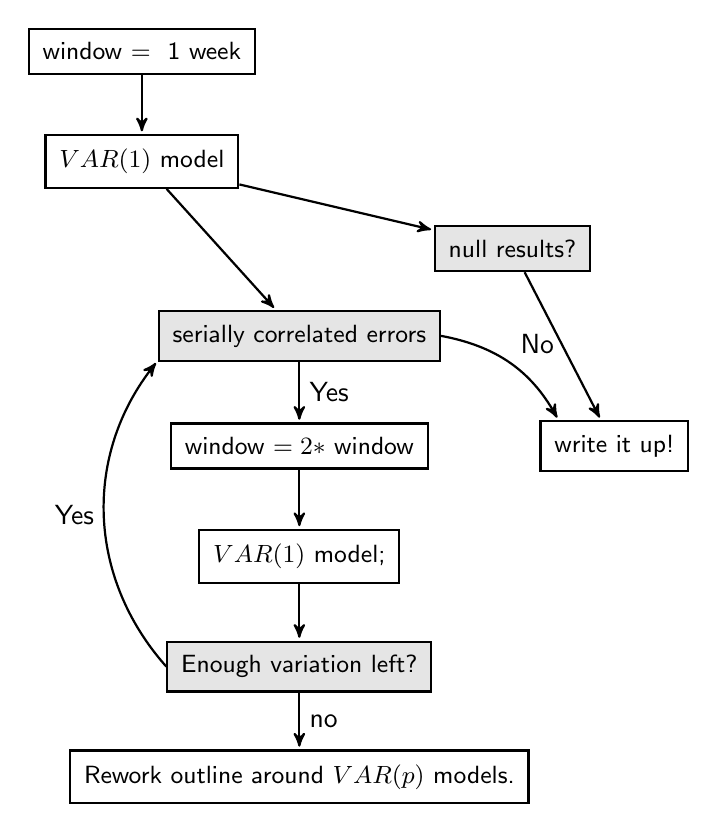
\begin{tikzpicture}  [->,>=stealth',shorten >=1pt,auto,
  thick,
  obs/.style={rectangle,draw,font=\sffamily\small,inner sep=0.5em},
      latent/.style={rectangle,draw,font=\sffamily\small,fill=gray!20, inner sep=0.5em},
      label/.style={font=\scshape\small},
      obsmic node/.style={ellipse,draw,font=\sffamily\small},
      unobsmic node/.style={ellipse,draw,font=\sffamily\small,fill=gray!20}]

      \node[obs] (t0) [] {window$~=~$ 1 week};

      \node[obs] (var1) [below of=t0,yshift=-0.4cm] {$VAR(1)$ model};

      \node[latent] (null1) [below right of=var1, yshift=-0.4cm, xshift=4cm] {null results?};

      \node[latent] (serial) [below left of=null1, yshift=-0.4cm, xshift=-2cm] {serially correlated errors};
      
      \node[obs] (increase_t) [below of=serial,yshift=-0.4cm] {window~$=2*$~window};
      
      \node[obs] (var2) [below of=increase_t,yshift=-0.4cm] {$VAR(1)$ model;};

      \node[latent] (null2) [below of=var2,yshift=-0.4cm] {Enough variation left?};

      \node[obs] (write) [right of=increase_t,xshift=3cm] {write it up!};

      \node[obs] (reoutline) [below of=null2,yshift=-0.4cm] {Rework outline around $VAR(p)$ models.};

      \path[every node/.style={font=\sffamily}]
      (t0) edge [] node {} (var1)
      (var1) edge [] node {} (null1)
      (var1) edge [] node {} (serial)
      (null1) edge [] node {} (write)
      (serial) edge [] node {Yes} (increase_t)
      (increase_t) edge [] node {} (var2)
      (var2) edge [] node {} (null2)
      (null2) edge [] node {no} (reoutline)
      (null2.west) edge [bend left=40] node {Yes} (serial.190)
      (serial.east) edge [bend left=25] node {No} (write.155);

\end{tikzpicture}



%%% Local Variables:
%%% mode: latex
%%% TeX-master: t
%%% End:

  \caption{Flow chart showing planned decision tree for iterating on selecting a time window. \label{fig:analytic_plan}}
\end{figure}

If we can't find a length of window without serial correlation then we can continue by extending our models using $VAR(p)$ models that have multiple time lags. The disadvantages of this are that we now have to infer many more parameters, we have to choose $p$ (this isn't so bad using information-theoretic model selection), and hypothesis tests become more complicated because we can model more complex relationships that are different on different time scales. While ecological relationships can be interpreted directly from the coefficient matrix $B$ of a $VAR(1)$ model, for a $VAR(p)$ model we'll have to inspect impulse response functions and decide how we'll draw conclusions about our hypotheses if we find relationships like short-run competition but long-run mutualism.  Figure \ref{fig:analytic_plan} summarizes this decision process.

\subsection{Hypothesis tests}
\label{sec:hypothesis_tests}

One complication in our analytic plan is that we test hypotheses about the relationship between generalists and specialists and our data only includes a handful of each.  Limited sample size means we can't infer the general relationship between types of groups and coefficients in the community matrix.  But we still have to average across all the dyads to test our hypotheses. Since we are Bayesians we can sum over posterior draws for each of the parameters in the community matrix that are relevant for a hypothesis test to generate a posterior distribution of the average.  

\subsubsection{\textbf{H1:} Competition between generalists}

We test \textbf{H1} by averaging over the marginal posteriors of elements $b_{i,j}$ of $B$ such that subreddits $i$ and $j$ are both generalists to calculate $\overline{b_{gen,gen}}$, the average relationship between generalists. 
We say that our analysis supports \textbf{H1} if the 95\% credible interval of $\overline{b_{gen,gen}}$ is strictly negative.


\subsubsection{\textbf{H2:} Generalists benefit specialists}

We test \textbf{H2} by averaging over the marginal posteriors of elements $b_{i,j}$ of $B$ such that subreddit $i$ is a generalist and subreddit $j$  is a specialist, to calculate $\overline{b_{gen,spec}}$, the average influence of a generalist on a specialist. We say that our analysis supports \textbf{H2} if the 95\% credible interval of $\overline{b_{gen,spec}}$ is strictly positive.


\subsubsection{\textbf{H3:} Commensalism between generalists and specialists}

We test \textbf{H2} by averaging over the marginal posteriors of elements $b_{i,j}$ of $B$ such that subreddit $i$ is a specialist and subreddit $j$  is a generalist, to calculate $\overline{b_{spec,gen}}$, the average influence of a specialist on a generalist. We say that our analysis supports \textbf{H2} if the 95\% credible interval of $\overline{b_{gen,spec}}$ contains 0 and is less than the absolute value of  $\overline{b_{gen,spec}}$.  This means that a strictly commensal relationship is plausible and that the average influence of specialists on generalists is very likely weaker than that of generalists on specialists.

\section{Ethical Concerns}

This study bears the usual ethical concerns of observational research in public online spaces.  Participants in Reddit communities are unlikely to expect that traces of their behavior will be analyzed in studies like this one.  

The data we're using is very minimal as it only includes aggregate counts of activities.  Those individuals who are most active in the smaller communities we study might feel exposed to scrutiny as they may identify with those communities.  Participants in these communities might be sensitive to connotations that their communities compete with or benefit from latent ecological relationships to other communities.  

%Organizational ecologists \citet{hannan_logics_2007} argue that ecological dynamics between organizations depend on the ``audiences'' of organizations by which they mean groups like investors, employees, and consumers.  In applying this thinking to generalization and specialization of online communities, we proposes that for a specialist community to survive it must have an audience of participants who prefer to participate in the specialist community over the other.  

\section{Dummy findings, tables, visualizations}

\begin{table}[h]
\begin{tabular}{l|c c c}
  subreddit & mean & sd & boxplot \\ \hline

  /r/Seattle & 40 & 20 & \raisebox{-0.5\totalheight}{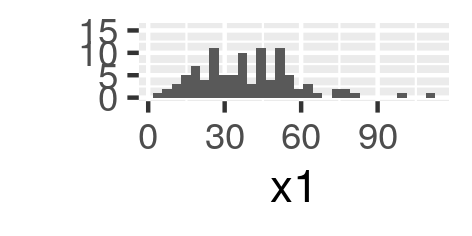
\includegraphics[width=4cm, height=2cm]{resources/random_dist.png}}
\end{tabular}
\caption{Table of time-averaged summary statistics and distributions for each community.}
\end{table}

\begin{figure}[h]
  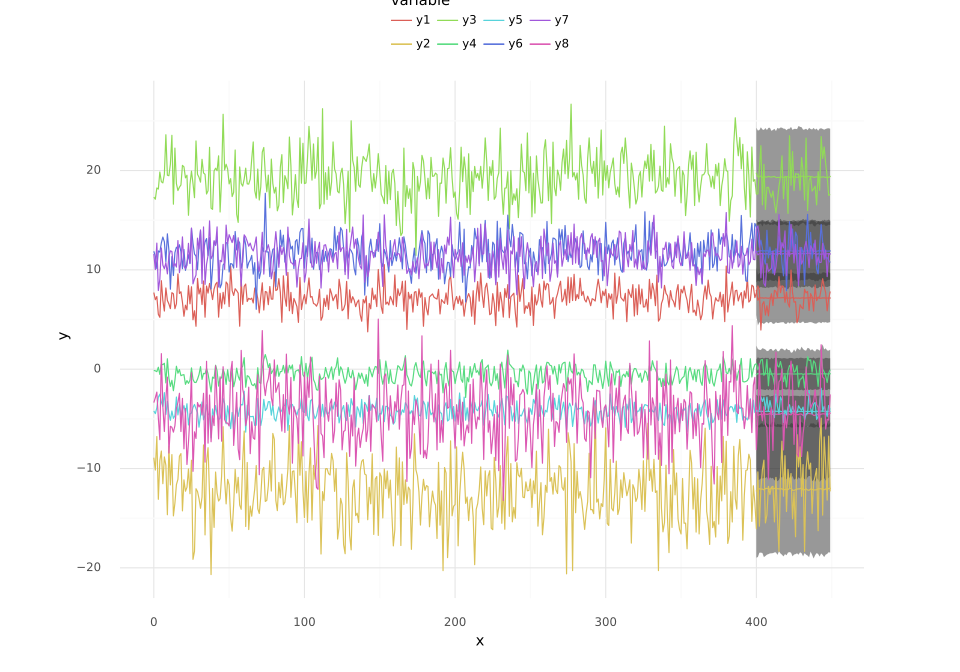
\includegraphics[width=\textwidth]{resources/example_forecast.png}
  \caption{One or more plots presenting raw time series data with our model fit and forecast}
\end{figure}
\clearpage

\begin{table}[h]
\footnotesize
\begin{tabular}{l | c c c c}
  & seattle & seattlewa & seattlebike & seattleents \\ \hline
  seattle & 0.50 (0.45, 0.55) & -0.30 (-0.35, -0.23) & 0.20 (0.1, 0.3) & 0.30 (0.04, 0.4) \\
  seattlewa & -0.50 (-0.8,-0.1) & 0.50 (0.43, 0.58) & 0.10 (0.02, 0.20) & 0.20 (0.10, 0.30) \\
  seattlebike & 0.010 (-0.2, 0.2) & -0.040 (-0.10, 0.20) & -0.01 (-0.70, 0.80) & 0.10 (0.05, 0.15) \\
  seattleents & 0.020 (-0.23, 0.4) & 0.040 (0.01, 0.23) & -0.01 (-0.30, 0.20) & 0.20 (0.08, 0.25) \\ \hline
\end{tabular}
\caption{Table showing estimated community matrix with 95\% credible intervals}
\end{table}

% bibliography here
\setcounter{biburlnumpenalty}{9001}
\printbibliography[title = {References}, heading=secbib]


\end{document}

%  LocalWords: commensalism commensal mutualism predation subreddit Reddit subreddits
